\section{Bold simulator}
\subsection*{2.a)}
\subsection*{2.b)}
\subsection*{2.c)}
\subsubsection*{1}
Til verificering af den diskrete model kan man fx. løse de givne ligninger for den matematiske model
eksakt og se hvorvidt denne og den diskrete approksimation udvikler sig tilnærmelsesvist ens.

Dette er naturligvist ikke tilfældet for alle differentialligninger, men det er her muligt da ligningen
er tilpas simpel:
\begin{align}
x''(t) 	&= 0 \\
x'(t) 	&= v_{x,0} \\
x(t) 	&= t \cdot v_{x,0} + x_0 
\end{align}
\begin{align}
y''(t)	&= -g \\
y'(t)	&= -g \cdot t + v_{y,0} \\
y(t)	&= \frac{-1}{2} \cdot g \cdot t + v_{y,0} \cdot t + y_0
\end{align}

Til validering af simulatoren kunne man optage kastet af en bold (her gerne i et rum med vakuum\ldots)
og måle dennes position henad tidsaksen og aflede hastigheden til de forskellige punkter.
Derefter kunne man plotte disse data ind i simulatoren, og se om denne giver et tilfredstillende output,
altså et output der passer til den indsamlede data.

Man kunne også, i mangel på kamera, opstille nogle fornuftige hypoteser om hvordan simulatoren skal
opføre sig når man ``skruer'' på de givne variable. Nogle eksempler:
\begin{itemize}
\item ændring af $m$ burde ikke have nogen indflydelse på vores simulation, da modellen er for simple
til at massen spiller en rolle.
\item ændring af $g$ burde gøre at hastigheden ud af y-aksen ($v_y$) per tidsenhed ($\Delta t$) ændres,
hvor en højere $g$ skulle resultere i en større ændring imod en lavere $g$.
\item ændring af $\Delta t$ burde kun have betydning for hvor ``finkornet'' vores simulation er, dvs.
at hastigheden med hvilken tiden flyder ikke burde have nogen indflydelse på den her underliggende
model, men kun på hvor store stridt vi tager i simulationen.
Da simulationen er en diskret approksimation betyder dette at en mindre $\Delta t$ vil give en højere
præcision, dvs. flere datapunkter fra startkast til at bolden rammer jorden.
\end{itemize} 
\subsubsection*{2}
For at afprøve vores hypoteser starter vi først med at have et basiseksperiment,
hvor $m = 1, g = 9.81, \Delta t = 0.01, x_0 = 0, y_0 = 1, v_{x,0} = 2, v_{y,0} = 2$.
Resultatet kan ses på figur \ref{basis}.

Vi starter ud med at skrue på massen $m$ til hhvs. $0.5$ og $2$, en fordobling og en halvering.
Vi får her som ventet præcis den samme kurve som basiseksperimentet, hvorfor vi ikke fremviser
to ekstra ens figurer.

Vi skruer nu på tyngdeaccelerationen $g$ til hhvs. $4.905$ og $19.62$, igen en fordobling og en halvering.
Resultatet kan ses på figur \ref{lessg} og \ref{moarg}.
Vi ser her at ved lavere tyngdeacceleration flyver bolden længere og ved højere tyngdeacceleration falder
bolden hurtigere til jorden.

Vi skruer nu til sidst på $\Delta t$ til hhvs. $0.08$ og $0.00125$, her gange hhvs. dividere vi med 8 for
at gøre forskellen mere tydelig.
Resultatet kan ses på figur \ref{lesst} og \ref{moart}.
Det er tydeligt at der er færre hhvs. flere datapunkter når vi gør $\Delta t$ større hhvs. mindre.

Vores hypoteser om vores simulation holder altså. Kurven for boldens bane opføre sig som forventet
under forskellige fysiske forhold, og simulationen kan siges at være god ud fra vores forsimplede
model af verdenen. Den holder selvfølgelig ikke i mere komplicerede sammenhæng (fx. med vindmodstand mm.)
men det er heller ikke det den er bygget til at simulere.

\begin{figure}
\centering
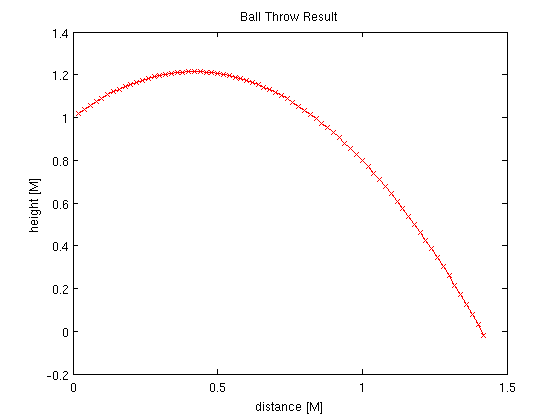
\includegraphics[scale=0.75]{basisrun}
\caption{Basiseksperiment\label{basis}}
\end{figure}

\begin{figure}
\centering
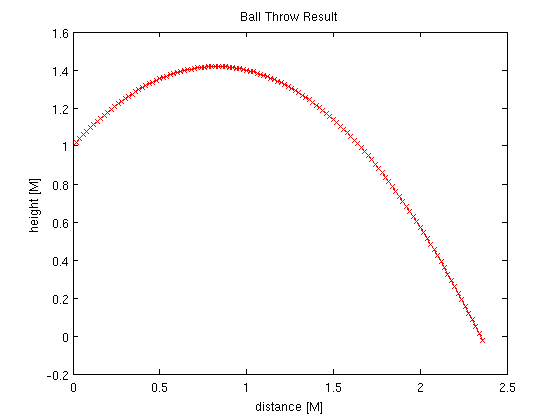
\includegraphics[scale=0.75]{lessgravity}
\caption{$g = 4.905$ \label{lessg}}
\end{figure}

\begin{figure}
\centering
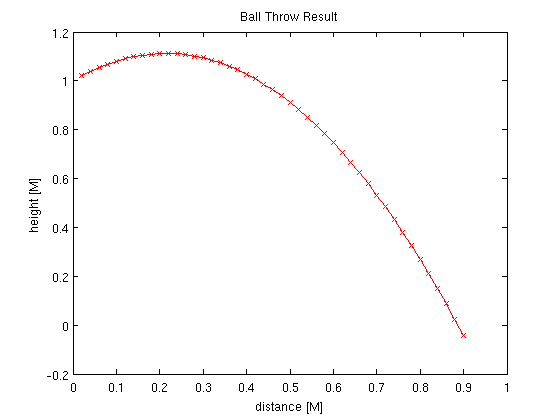
\includegraphics[scale=0.75]{moargravity}
\caption{$g = 19.62$ \label{moarg}}
\end{figure}

\begin{figure}
\centering
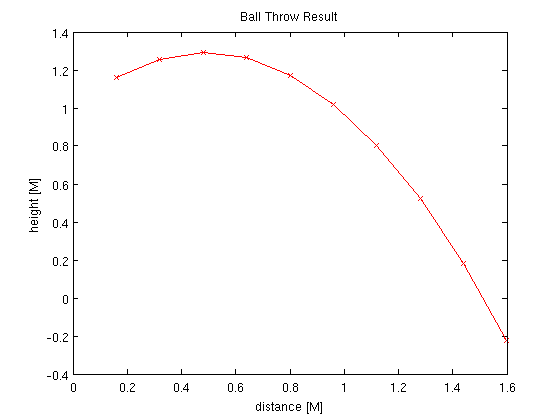
\includegraphics[scale=0.75]{lesstime}
\caption{$\Delta t = 0.08$ \label{lesst}}
\end{figure}

\begin{figure}
\centering
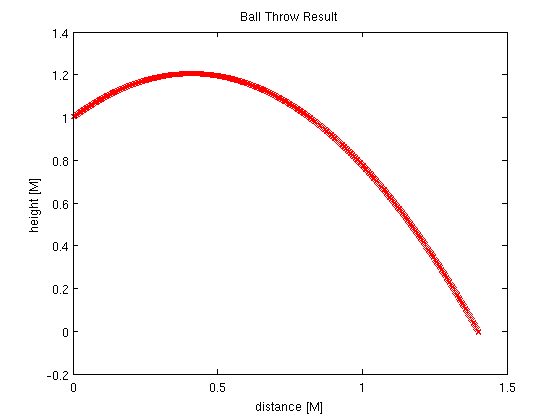
\includegraphics[scale=0.75]{moartime}
\caption{$\Delta t = 0.00125$ \label{moart}}
\end{figure}
